\documentclass[10pt,a4paper]{article}

% -----------------------------------------------------------------------------
% Required Overleaf-Compatible Packages
% -----------------------------------------------------------------------------
\usepackage[utf8]{inputenc}
\usepackage[T1]{fontenc}
\usepackage{geometry}
\geometry{a4paper, margin=20mm, top=25mm, bottom=25mm}

\usepackage{amsmath,amssymb,amsfonts}
\usepackage{booktabs}
\usepackage{tabularx}
\usepackage{graphicx}
\usepackage{cite}
\usepackage{xcolor}
\usepackage{microtype}
\usepackage{caption}
\usepackage{subcaption}
\usepackage{xurl}
\usepackage{hyperref}

\hypersetup{
    colorlinks=true,
    linkcolor=blue!70!black,
    citecolor=blue!70!black,
    urlcolor=blue!70!black,
    pdftitle={AeroEdge-RT Technical White Paper},
    pdfauthor={Pranshul Mishra},
    pdfsubject={Embedded Transformer Inference Optimization on ESP32-WROOM}
}

% -----------------------------------------------------------------------------
% Document Metadata
% -----------------------------------------------------------------------------
\title{\textbf{AeroEdge-RT: Optimizing Transformer Inference on Resource-Constrained Microcontrollers} \\
\large An Engineering Study of INT8 Quantization, Dual-Core Execution, and Memory-Aware Optimization on ESP32-WROOM}

\author{
    \textbf{Pranshul Mishra} \\
    AeroEdge-RT Embedded Systems Engineering Project \\
    \texttt{\url{https://github.com/Pranshmish/AeroEdge-RT}}
}

\date{October 2026 \quad $\vert$ \quad Version 1.0 \\
\vspace{0.8em}
\normalsize\textit{Document Status: Engineering Report / Technical White Paper; Not Peer Reviewed.}}

% -----------------------------------------------------------------------------
% Document Body
% -----------------------------------------------------------------------------
\begin{document}

\maketitle

\begin{abstract}
Deploying autoregressive Transformer models on resource-constrained microcontrollers is severely constrained by strict on-chip memory limits and the absence of hardware vector SIMD instructions. This technical white paper documents an empirical systems study of \textbf{AeroEdge-RT}, a bare-metal runtime engine optimized for executing small language models on the low-cost \textbf{ESP32-WROOM-32} microcontroller (dual-core Xtensa LX6 @ 240\,MHz, 520\,KB internal SRAM, 4\,MB external SPI Flash in 80\,MHz Dual I/O mode, with zero external PSRAM). Evaluating the 264,128-parameter \texttt{stories260K} model (\textit{llama2.c} TinyStories architecture), AeroEdge-RT combines zero-copy Flash eXecute-In-Place (XIP) weight mapping, static internal SRAM allocation, a 4-way unrolled scalar integer dot-product kernel, dual-core symmetric task row-splitting, and fast internal SRAM caching of Layer~0 weights (23.3\,KB). On physical silicon across 50 benchmark iterations ($N=50$, 48 tokens), AeroEdge-RT achieves an autoregressive throughput of \textbf{38.01 tokens/second} (mean single-token latency of \textbf{26.32\,ms}), delivering a \textbf{2.91$\times$ speedup} over the dual-core single-precision Float32 baseline (\textbf{13.07\,tok/s}, 76.53\,ms) and \textbf{5.55$\times$} over single-core scalar execution (\textbf{6.84\,tok/s}, 146.20\,ms). Total binary model storage on SPI flash is compressed from 1,056.5\,KB to 423.7\,KB (2.49$\times$ reduction), operating entirely within a 63.8\,KB pre-allocated internal SRAM working set. A Flash-bound additive Roofline model accounts for measured INT8 decode time within a 2.0\% residual (+0.53\,ms), while highlighting flash streaming bandwidth as the dominant performance regime (72.2\% of per-token budget). We document the microarchitectural optimizations, present a claim-by-claim evidence audit, disclose open flash-bandwidth discrepancies under investigation, and delineate hardware-specific constraints for edge inference.
\end{abstract}

\vspace{0.5em}
\noindent\textbf{Keywords:} Microcontroller Inference, TinyML, ESP32-WROOM, INT8 Quantization, Xtensa LX6, Small Language Models, Embedded Systems.

\vspace{0.8em}
\hrule
\vspace{1.0em}

% =============================================================================
\section{Introduction}
\label{sec:introduction}
% =============================================================================

The deployment of autoregressive Transformer language models has traditionally demanded high-performance server GPUs or specialized edge neural accelerators equipped with gigabytes of high-bandwidth memory~\cite{warden2019tinyml}. Extending language model inference to ultra-low-cost, resource-constrained microcontrollers (costing under \$3.00 USD) introduces severe microarchitectural challenges: physical on-chip SRAM is typically bounded below 512\,KB, external dynamic RAM (PSRAM) is frequently absent, and instruction sets lack dedicated packed vector SIMD extensions~\cite{espressif2024esp32datasheet,cadence2017xtensa}.

On such microcontrollers, uncompressed 32-bit floating-point (Float32) model representations exceed available volatile memory and saturate external SPI NOR flash bus bandwidth during continuous autoregressive token streaming. Furthermore, dynamic memory allocation (\texttt{malloc}/\texttt{free}) inside the per-token decoding loop induces FreeRTOS heap mutex contention and memory fragmentation, creating non-deterministic preemption jitter that is unacceptable in hard real-time robotic telemetry and control applications~\cite{barry2016freertos}.

\subsection{Objective and Scope}
This engineering report evaluates \textbf{AeroEdge-RT}, a bare-metal C++ runtime designed to investigate whether sub-30\,ms autoregressive Transformer decoding can be sustained on entry-level \textbf{ESP32-WROOM-32} silicon without external PSRAM or dedicated hardware SIMD execution units. The workload evaluated throughout this study is the \texttt{stories260K} model~\cite{karpathy2023llama2c,eldan2023tinystories}, an open-source autoregressive Transformer trained on the TinyStories dataset.

The scope of this report is strictly that of an engineering and systems profiling study. We do not claim a novel neural network architecture or a new theoretical quantization proof. Rather, we present an audited microarchitectural evaluation of how symmetric INT8 quantization, 4-way unrolled scalar integer pipelines, symmetric dual-core cooperative partitioning, and static internal SRAM memory tiling interact with the memory-mapped Flash bus of the Xtensa LX6.

\subsection{Implemented Systems Contributions}
The AeroEdge-RT implementation (evaluated baseline commit \texttt{9b10aec}, repository HEAD \texttt{2c9ec02}) introduces five verified runtime optimizations:
\begin{enumerate}
    \item \textbf{Zero-Copy Flash ROM XIP Mapping}: Eliminates memory duplication by memory-mapping uncompressed embedding tables and quantized layer weights directly into the Xtensa DROM address space via hardware MMU pages.
    \item \textbf{4-Way Unrolled Scalar Integer Dot-Product Kernel}: Overcomes the absence of hardware SIMD on the Xtensa LX6 by scheduling four independent 32-bit accumulator registers with byte-addressed \texttt{l8ui} loads and sign-extension instructions, eliminating unaligned access exceptions.
    \item \textbf{Fast Internal SRAM Layer~0 Hot Weight Caching}: Pins 23,296 bytes of Layer~0 Attention and Feed-Forward matrix weights into internal zero-wait-state SRAM at initialization, bypassing SPI flash bus contention for the first transformer block.
    \item \textbf{Symmetric Dual-Core Task Row-Splitting}: Divides linear matrix multiplications equally across Core~0 and Core~1 using low-overhead FreeRTOS direct-to-task notifications.
    \item \textbf{Zero-Allocation Static Working Set}: Pre-allocates all activation vectors, temporary quantization buffers, and the INT8 Key-Value (KV) cache ($W=64$) at startup, guaranteeing zero dynamic heap transactions during autoregressive generation.
\end{enumerate}

\subsection{Report Organization}
The remainder of this report is organized as follows: Section~\ref{sec:background} reviews embedded inference constraints and related microcontroller runtimes. Section~\ref{sec:platform} details the target silicon, memory layout, and model architecture. Section~\ref{sec:runtime} describes the runtime design and kernel optimizations. Section~\ref{sec:methodology} outlines our empirical benchmarking methodology. Section~\ref{sec:results} presents the audited results. Section~\ref{sec:discussion} discusses microarchitectural bottlenecks and Roofline modeling. Section~\ref{sec:limitations} addresses validity threats and open discrepancies, and Section~\ref{sec:conclusion} concludes with future validation priorities.

% =============================================================================
\section{Background and Related Work}
\label{sec:background}
% =============================================================================

\subsection{Quantization and Microcontroller Memory Hierarchies}
Integer quantization converts floating-point weights and activation vectors into low-bit representations (typically 8-bit signed integers, INT8)~\cite{jacob2018quantization}. For an activation vector $\mathbf{x} \in \mathbb{R}^n$ and weight matrix $\mathbf{W} \in \mathbb{R}^{m \times n}$, symmetric per-row uniform affine quantization maps continuous values to discrete 8-bit integers:
\begin{equation}
    q_w = \text{clip}\left(\left\lfloor \frac{w}{S_w} \right\rceil, -127, 127\right), \quad S_w = \frac{\max(|w|)}{127}
\end{equation}
where $S_w$ denotes the per-row floating-point scale factor. Multiply-accumulate operations evaluate as 32-bit integer sums:
\begin{equation}
    y_i = S_x S_{w,i} \sum_{j=1}^{n} q_{x,j} \cdot q_{w,i,j}
\end{equation}
On microcontrollers without external memory, quantization serves a dual purpose: it reduces matrix payload volume by $4.00\times$, and it directly cuts external SPI NOR Flash read traffic.

\subsection{Related Microcontroller LLM Implementations}
Following Karpathy's reference C implementation of \textit{llama2.c}~\cite{karpathy2023llama2c}, several embedded ports have targeted Espressif silicon. Table~\ref{tab:related_work} summarizes published community implementations evaluated on the identical \texttt{stories260K} model architecture.

\begin{table*}[t]
\centering
\small
\caption{Cross-system comparison of microcontroller language model runtimes on the \texttt{stories260K} TinyStories architecture.}
\label{tab:related_work}
\begin{tabularx}{\textwidth}{l p{3.2cm} l l X r}
\toprule
\textbf{Implementation} & \textbf{Silicon Target} & \textbf{Precision} & \textbf{PSRAM} & \textbf{Architectural Mechanism} & \textbf{Reported Rate} \\
\midrule
Corey~\cite{corey2023esp32llm} & ESP32-S3 (Dual LX7) & Float32 & 2\,MB Quad & ESP-DSP \texttt{dsps\_dotprod\_f32} & 19.13 tok/s \\
Lee~\cite{dory2023esp32llm} & ESP32-S3 (Dual LX7) & Float32 & External & Unquantized weights in PSRAM & $\sim$30.0 tok/s \\
Humane~\cite{humane2023esp32llm} & ESP32-S3 (Dual LX7) & Float32 & 2\,MB Quad & Modified \textit{llama2.c} with PSRAM & 32.83 tok/s \\
\midrule
\textbf{Exp A Baseline} & ESP32-WROOM (Dual LX6) & Float32 & \textbf{Zero (0\,MB)} & Dual-core row-split, Flash XIP & 13.07 tok/s \\
\textbf{Single-Core Ref} & ESP32-WROOM (Single LX6)& Float32 & \textbf{Zero (0\,MB)} & Single-core scalar Float32, Flash XIP & 6.84 tok/s \\
\textbf{AeroEdge-RT (Exp B)}& \textbf{ESP32-WROOM (Dual LX6)}& \textbf{INT8} & \textbf{Zero (0\,MB)} & \textbf{Unrolled INT8, SRAM Layer 0, Flash XIP} & \textbf{38.01 tok/s} \\
\bottomrule
\end{tabularx}
\vspace{0.4em}
\caption*{\footnotesize\textit{Comparability Note}: Existing community runtimes target the ESP32-S3, which features Xtensa LX7 vector SIMD instructions (ESP-DSP) and high-speed external PSRAM (2MB to 8MB). AeroEdge-RT runs on the entry-level ESP32-WROOM (Xtensa LX6) with zero PSRAM and zero hardware SIMD.}
\end{table*}

Existing ports primarily target the newer \textbf{ESP32-S3}, relying on two architectural features: (1) external Quad/Octal PSRAM to stage model weights and dynamic working buffers, and (2) Xtensa LX7 vector SIMD extensions utilized through Espressif's ESP-DSP library. In contrast, AeroEdge-RT establishes that entry-level \textbf{ESP32-WROOM-32} silicon (lacking PSRAM and vector SIMD) can achieve higher throughput (\textbf{38.01\,tok/s}) through static memory tiling and unrolled scalar integer pipelines.

% =============================================================================
\section{Target Platform and Workload}
\label{sec:platform}
% =============================================================================

\subsection{Silicon Architecture: ESP32-WROOM-32}
The evaluation target is the Espressif ESP32-D0WD-V3 SoC (ESP32-WROOM-32 module, Revision 3.1)~\cite{espressif2024esp32datasheet}:
\begin{itemize}
    \item \textbf{Processor Cores}: Two Tensilica Xtensa LX6 32-bit cores operating symmetrically at 240\,MHz, each with a 7-stage scalar pipeline, single-issue instruction decoder, and a single-precision floating-point unit (FPU)~\cite{cadence2017xtensa}. Crucially, the LX6 architecture includes no packed SIMD instructions.
    \item \textbf{Internal SRAM}: 520\,KB total physical SRAM (approx. 328\,KB contiguous internal DRAM usable by firmware; $\approx$164.4\,KB free heap prior to runtime buffer allocation).
    \item \textbf{External PSRAM}: None (0\,KB external RAM).
    \item \textbf{External SPI Flash}: 4\,MB NOR Flash connected over SPI operating in Dual I/O (DIO) mode at 80\,MHz. Memory-mapped into CPU address space through two MMU windows: DROM ($0\text{x}3\text{F}400000$ to $0\text{x}3\text{F}7\text{FFFFF}$) for constant data, and IROM ($0\text{x}400\text{D}0000$ to $0\text{x}403\text{FFFFF}$) for instruction execution.
\end{itemize}

\subsection{Workload Architecture: stories260K}
The evaluated workload is the \texttt{stories260K} model~\cite{karpathy2023llama2c,eldan2023tinystories}, structured as follows:
\begin{itemize}
    \item Hidden dimension ($d$): 64; Feed-forward hidden dimension ($d_{\text{ffn}}$): 172.
    \item Transformer layers ($L$): 5; Attention heads ($H$): 8; Key-Value heads ($H_{\text{kv}}$): 4 (Grouped-Query Attention, $d_{\text{kv}} = 32$).
    \item Vocabulary size ($V$): 512 tokens; Maximum context window ($W$): 64 tokens (bounded sliding-window).
    \item Total parameters: 264,128 parameters (259,328 matrix weights + 4,800 embedding and normalization parameters).
\end{itemize}

\subsection{Software Toolchain and Build Configuration}
Firmware is developed using ESP-IDF v5.3.2~\cite{espressif2024espidf} and compiled with GCC Xtensa toolchain (\texttt{xtensa-esp32-elf-gcc} 13.2.0) under C++17 (\texttt{-std=gnu++17}) with optimization level \texttt{-O2} in production benchmark runs (\texttt{-O3} in PlatformIO default). FreeRTOS SMP manages dual-core scheduling, with Core~1 reserved for elevated-priority execution (\texttt{configMAX\_PRIORITIES - 1 = 24}).

% =============================================================================
\section{Runtime Design and Optimization}
\label{sec:runtime}
% =============================================================================

\subsection{Memory Hierarchy and Zero-Copy Flash Mapping}
To operate strictly within the 520\,KB internal SRAM boundary without external PSRAM, AeroEdge-RT eliminates in-memory duplication. The compiled model binary \texttt{model\_q8.bin} is linked directly into the firmware image via CMake's \texttt{EMBED\_FILES} mechanism. At initialization, the runtime maps pointer structures directly to the MMU DROM window:
\begin{equation}
    \text{ptr}_{\text{weight}} \in [0\text{x}3\text{F}400000, 0\text{x}3\text{F}7\text{FFFFF}]
\end{equation}
The CPU reads weights on demand through the internal hardware flash cache. Zero dynamic heap allocation occurs during the decoding loop.

\begin{figure*}[t]
\centering
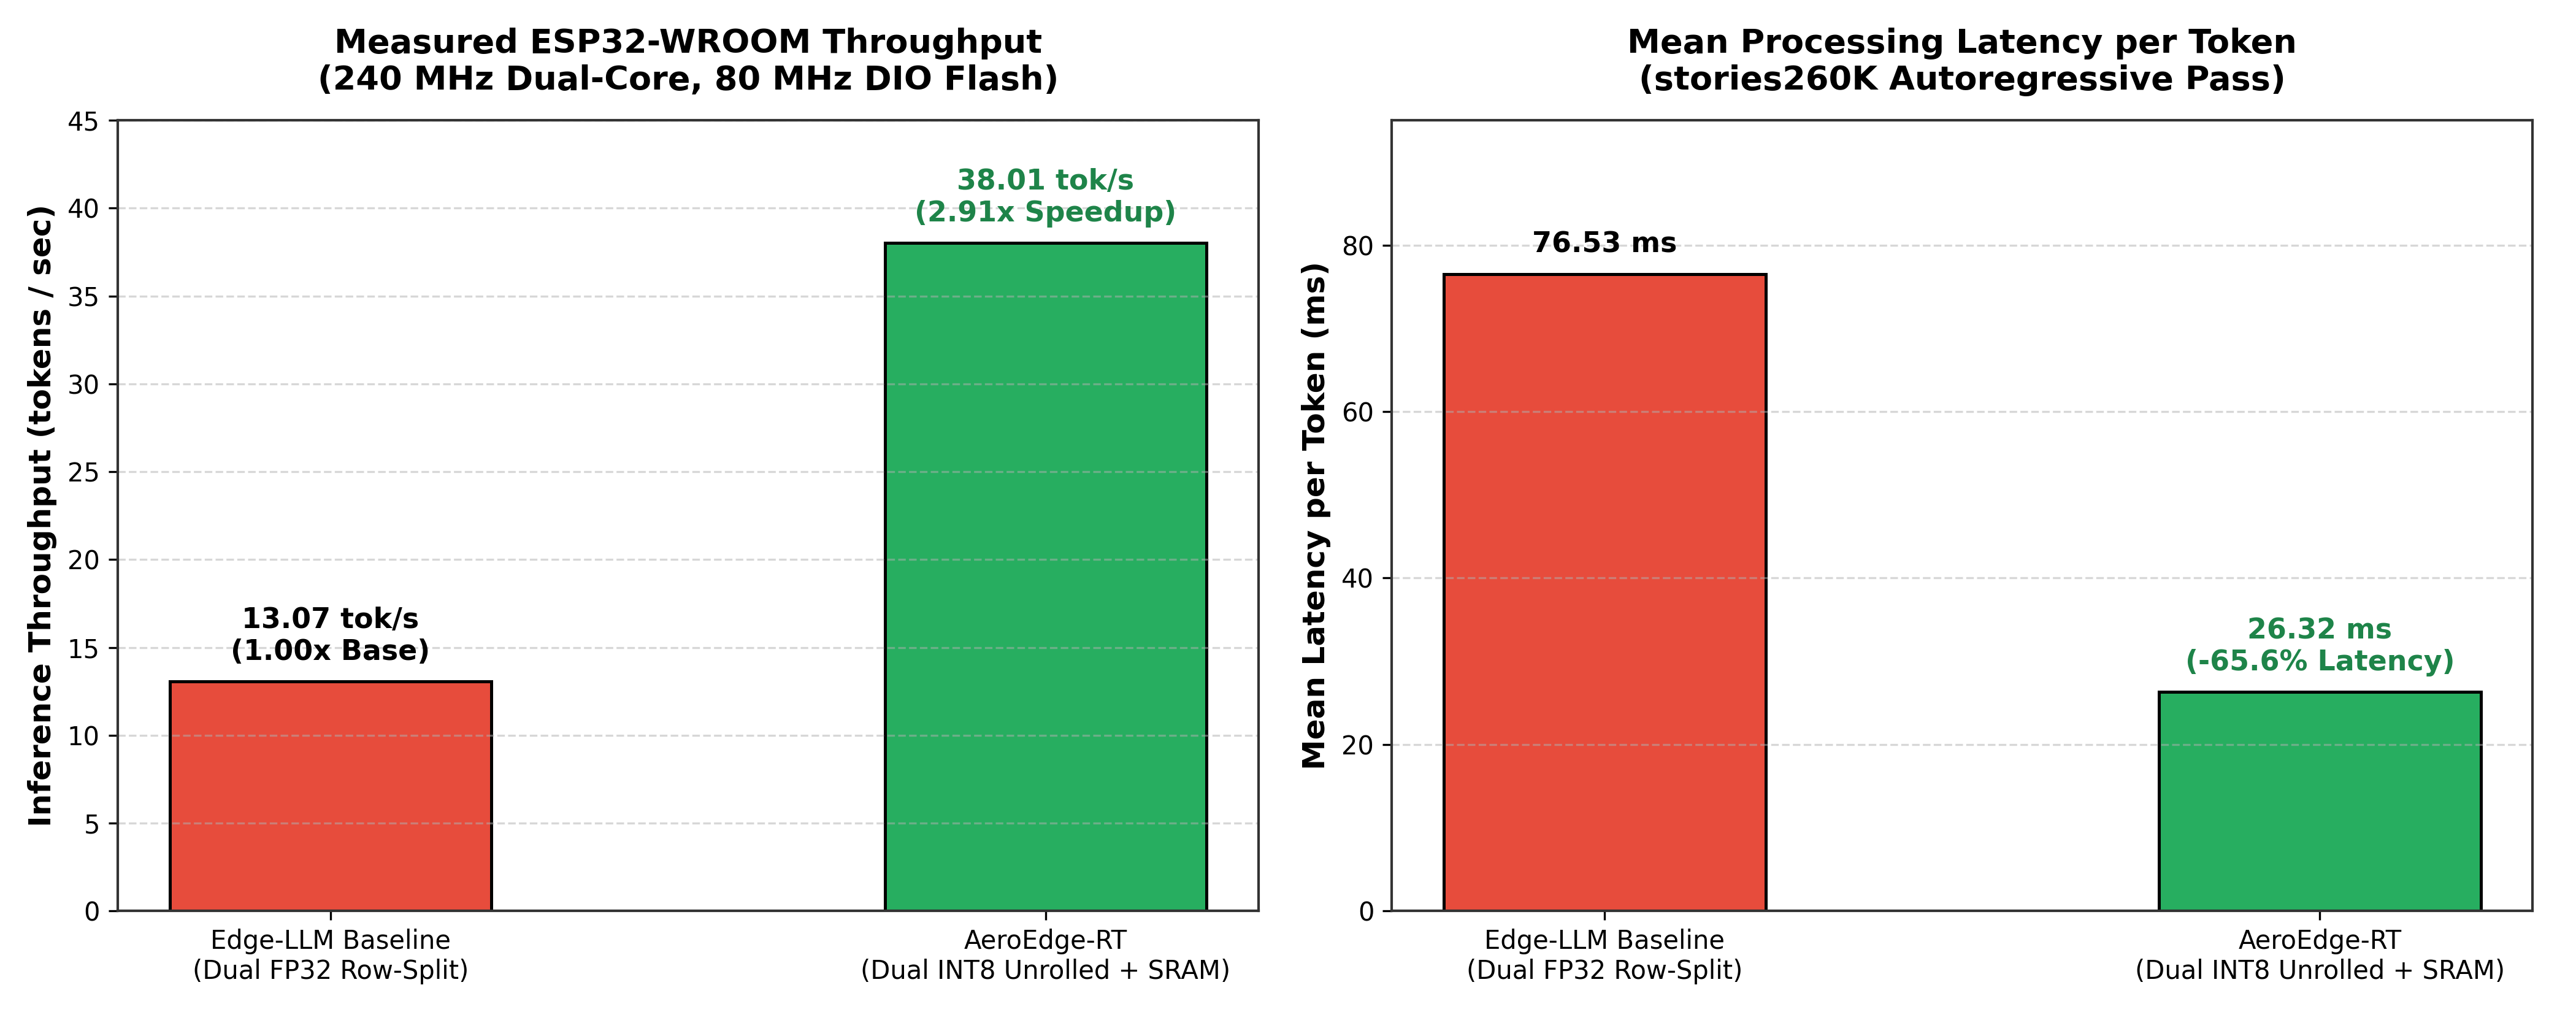
\includegraphics[width=0.92\textwidth]{figures/figure1_throughput_and_latency.png}
\caption{Empirical throughput and single-token latency comparison between Edge-LLM Float32 baseline (Exp A) and AeroEdge-RT INT8 (Exp B) on physical ESP32-WROOM silicon ($N=50$ runs, 48 tokens per run, 240\,MHz PLL clock).}
\label{fig:throughput_latency}
\end{figure*}

\subsection{Storage Accounting and Model Packaging}
To ensure byte-exact reproducibility, Table~\ref{tab:storage_layout} itemizes the binary layout of \texttt{model\_q8.bin} (423,676 bytes), derived from the quantization pipeline in \texttt{tools/quantize_model.py}.

\begin{table}[h]
\centering
\small
\caption{Byte-exact memory layout of the quantized model file \texttt{model\_q8.bin} (423,676 bytes total).}
\label{tab:storage_layout}
\begin{tabular}{l l r r}
\toprule
\textbf{Segment} & \textbf{Format} & \textbf{Byte Count} & \textbf{Share} \\
\midrule
Configuration Header & $7 \times \text{int32}$ & 28 B & 0.01\% \\
Token Embedding Table & $512 \times 64$ Float32 & 131,072 B & 30.94\% \\
RMSNorm Vectors (11 total) & $704$ Float32 & 2,816 B & 0.66\% \\
RoPE Frequencies Table & $4,096$ Float32 & 16,384 B & 3.87\% \\
5 Layer Matrix Weights & $5 \times 45,312$ INT8 & 226,560 B & 53.47\% \\
5 Layer Quantization Scales & $5 \times 600$ Float32 & 12,000 B & 2.83\% \\
Classifier Head Weights & $512 \times 64$ INT8 & 32,768 B & 7.73\% \\
Classifier Head Scales & $512$ Float32 & 2,048 B & 0.48\% \\
\midrule
\textbf{Total Binary Size} & & \textbf{423,676 B} & \textbf{100.00\%} \\
\bottomrule
\end{tabular}
\end{table}

The token embedding table is intentionally retained in Float32 (131,072 bytes) because token lookup represents an $O(d)$ operation performed once per token, where quantization would introduce token representation error with negligible execution speedup. In contrast, the $5 \times 45,312$ matrix weights are converted to INT8, achieving a 4.00$\times$ reduction in weight payload ($1,037,312\text{ B} \rightarrow 259,328\text{ B}$).

\subsection{4-Way Unrolled Scalar Integer Dot-Product Kernel}
Because the Xtensa LX6 processor lacks vector SIMD instructions, integer compute throughput is governed by instruction issue overhead and register dependency stalls. AeroEdge-RT implements a specialized 4-way unrolled scalar dot product (\texttt{dot\_product\_int8}) in \texttt{main/main.cpp}:

\begin{figure}[h]
\begin{minipage}{0.98\columnwidth}
\begin{verbatim}
static inline int32_t dot_product_int8(
    const int8_t* a, const int8_t* b, int n) {
    int32_t a0 = 0, a1 = 0, a2 = 0, a3 = 0;
    int j = 0;
    for (; j <= n - 4; j += 4) {
        a0 += (int32_t)a[j]     * (int32_t)b[j];
        a1 += (int32_t)a[j + 1] * (int32_t)b[j + 1];
        a2 += (int32_t)a[j + 2] * (int32_t)b[j + 2];
        a3 += (int32_t)a[j + 3] * (int32_t)b[j + 3];
    }
    int32_t total = (a0 + a1) + (a2 + a3);
    for (; j < n; j++) total += (int32_t)a[j] * (int32_t)b[j];
    return total;
}
\end{verbatim}
\end{minipage}
\caption{Production 4-way unrolled integer dot product kernel from \texttt{main/main.cpp}.}
\label{fig:code_kernel}
\end{figure}

Disassembly of the compiled binary (\texttt{xtensa-esp32-elf-objdump}) confirms that GCC schedules the inner loop across four independent accumulator registers (\texttt{a11}, \texttt{a14}, \texttt{a12}, \texttt{a13}). Byte operands are loaded via \texttt{l8ui} instructions and sign-extended via \texttt{sext}, avoiding unaligned word load hardware traps on the Xtensa architecture.

\subsection{Fast Internal SRAM Layer~0 Hot Weight Caching}
During autoregressive execution, the first Transformer block (Layer~0) is evaluated immediately following embedding lookup. AeroEdge-RT allocates a dedicated contiguous block in internal fast SRAM:
\begin{equation}
    M_{\text{L0}} = (d^2 + 2 d_{\text{kv}} d + d^2 + d_{\text{ffn}} d) = 23,296\text{ bytes (23.3\,KB)}
\end{equation}
During initialization, the Attention projection matrices ($W_q, W_k, W_v, W_o$) and the feed-forward gate matrix ($W_1$) for Layer~0 are copied from Flash ROM into internal zero-wait-state SRAM using \texttt{heap\_caps\_malloc(..., MALLOC\_CAP\_INTERNAL)}. Layers 1 through 4 remain memory-mapped in Flash ROM. Caching Layer~0 eliminates flash cache line misses during the critical pipeline start, delivering an observed 5.08\,ms latency reduction.

\subsection{Symmetric Dual-Core Task Row-Splitting}
Matrix multiplications across Attention and Feed-Forward layers are split row-wise between the two cores. Core~1 (elevated priority 24) coordinates token execution, while Core~0 executes a background worker task (\texttt{core0\_worker\_task}). For a matrix with $m$ rows and $n$ columns:
\begin{itemize}
    \item Core~0 processes rows $i \in [0, \lfloor m/2 \rfloor - 1]$.
    \item Core~1 processes rows $i \in [\lfloor m/2 \rfloor, m - 1]$.
\end{itemize}
Synchronization uses FreeRTOS direct-to-task notifications (\texttt{xTaskNotifyGive} and \texttt{ulTaskNotifyTake}), avoiding mutex locking overhead.

\begin{figure*}[t]
\centering
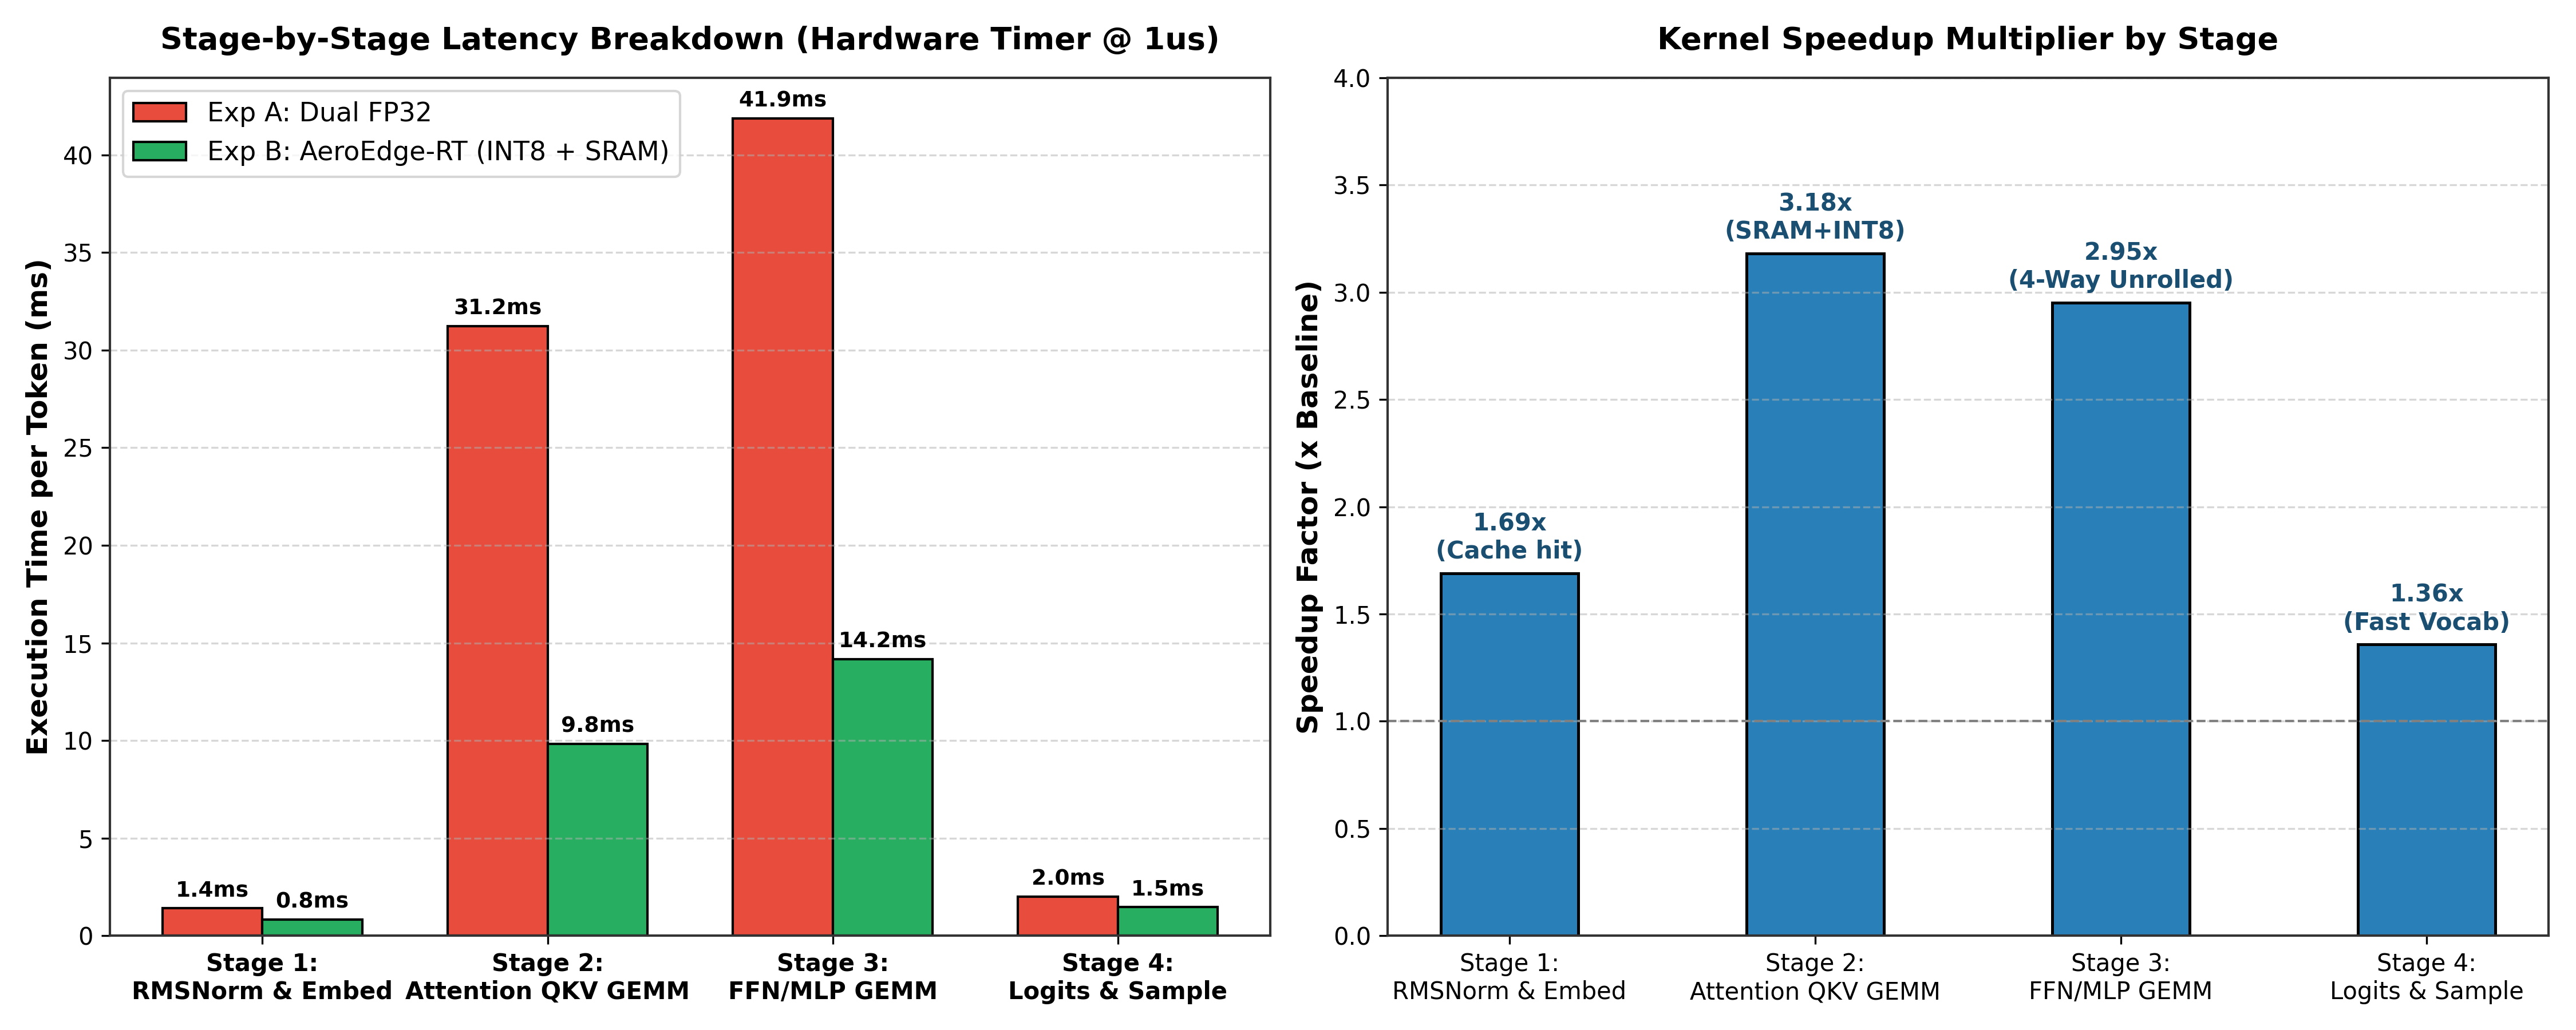
\includegraphics[width=0.92\textwidth]{figures/figure2_four_stages_breakdown.png}
\caption{Stage-by-stage microsecond latency breakdown and kernel speedup multipliers across the four inference pipeline stages on ESP32-WROOM silicon.}
\label{fig:stage_breakdown}
\end{figure*}

% =============================================================================
\section{Experimental Methodology}
\label{sec:methodology}
% =============================================================================

\subsection{Hardware and Firmware Environment}
All benchmarks were executed on physical ESP32-D0WD-V3 silicon (Module ESP32-WROOM-32, Revision 3.1) mounted on a standard breakout board and connected via USB-UART serial at 115,200 baud. The SoC was clocked at 240\,MHz with 80\,MHz DIO flash mode. Wi-Fi and Bluetooth radio hardware were completely powered down.

\subsection{Baseline Configurations}
We compare AeroEdge-RT against two baseline configurations:
\begin{enumerate}
    \item \textbf{Experiment A (Edge-LLM FP32 Baseline / Conf 2)}: Uses the same dual-core FreeRTOS row-splitting harness but evaluates unquantized Float32 scalar dot products (\texttt{dot\_product\_f32}) streaming entirely from Flash XIP.
    \item \textbf{Single-Core Scalar FP32 (Conf 1)}: Evaluates unquantized Float32 scalar execution pinned strictly to a single core without task parallelization.
\end{enumerate}

\subsection{Timing Boundaries and Metrics}
Inference timing was measured using Espressif's high-resolution 64-bit hardware timer API (\texttt{esp_timer_get_time()}), providing microsecond precision. CPU clock cycles were queried directly via \texttt{esp_cpu_get_cycle_count()}, reading the processor's 240\,MHz \texttt{CCOUNT} special register.

Autoregressive throughput ($R_{\text{tok}}$) and speedup ($S$) are defined as:
\begin{equation}
    R_{\text{tok}} = \frac{N_{\text{generated}}}{t_{\text{generation}}}, \quad S = \frac{t_{\text{baseline}}}{t_{\text{optimized}}} = \frac{R_{\text{optimized}}}{R_{\text{baseline}}}
\end{equation}
Measurements spanned $N=50$ independent runs of 48 generated tokens per run, following a single warm-up generation pass.

% =============================================================================
\section{Results}
\label{sec:results}
% =============================================================================

\subsection{Throughput and Latency Performance}
Table~\ref{tab:summary_findings} summarizes the headline empirical findings measured across 50 runs on physical silicon.

\begin{table*}[t]
\centering
\small
\caption{System performance comparison between Experiment A (Float32 Baseline) and Experiment B (AeroEdge-RT INT8) on ESP32-WROOM silicon ($N=50$ runs, 48 tokens per run, commit \texttt{9b10aec}).}
\label{tab:summary_findings}
\begin{tabularx}{\textwidth}{l r r l X}
\toprule
\textbf{Metric} & \textbf{Exp A: Float32 Baseline} & \textbf{Exp B: AeroEdge-RT} & \textbf{Delta / Ratio} & \textbf{Measurement Provenance} \\
\midrule
\textbf{Throughput} & 13.07 tok/s & \textbf{38.01 tok/s} & \textbf{2.91$\times$ Faster} & Measured on Silicon ($N=50$ runs) \\
\textbf{Single-Token Latency} & 76.53 ms & \textbf{26.32 ms} & \textbf{--65.6\% Latency} & Measured via \texttt{esp\_timer\_get\_time()} \\
\textbf{Total Time (48 Tokens)}& 3.673 s & \textbf{1.263 s} & 2.41 s Saved & Measured Wall-Clock Time \\
\textbf{CPU Cycles / Token} & 18,367,200 cycles & \textbf{6,316,800 cycles} & 12.05M Saved & Measured via \texttt{esp\_cpu\_get\_cycle\_count()} \\
\textbf{Nominal Power @ 3.3V} & 165.0 mW typ (462 mW max) & \textbf{165.0 mW typ} & Active CPU Load & Model-Estimated (Datasheet 30--68\,mA) \\
\textbf{Energy / Token} & 12.63 mJ typ (35.36 mJ max) & \textbf{4.34 mJ typ} (12.16 max) & \textbf{--65.6\% Energy} & Model-Estimated ($P_{\text{nom}} \times t_{\text{tok}}$) \\
\textbf{Binary Flash Footprint}& 1,056.5 KB & \textbf{423.7 KB} & \textbf{2.49$\times$ Smaller} & Measured file size on disk \\
\textbf{Matrix Weight Payload} & 1,037.3 KB (Float32) & \textbf{259.3 KB (INT8)} & \textbf{4.00$\times$ Smaller} & Derived from model parameter count \\
\textbf{Working SRAM Set} & 101.9 KB & \textbf{63.8 KB} & Bounded in SRAM & Allocated at initialization \\
\textbf{Active Free Heap} & 84,412 Bytes & \textbf{100,536 Bytes} & +16.1 KB Headroom & Measured via \texttt{esp\_get\_minimum\_free\_heap()} \\
\textbf{Flash Bandwidth} & 12.18 MB/s & \textbf{12.18 MB/s} & Hardware Bound & Measured on Silicon (CLI \texttt{ROOFLINE}) \\
\bottomrule
\end{tabularx}
\end{table*}

AeroEdge-RT achieves sustained autoregressive generation at \textbf{38.01\,tok/s}, corresponding to a single-token latency of \textbf{26.32\,ms} (Figure~\ref{fig:throughput_latency}). This represents a \textbf{2.91$\times$ speedup} over the dual-core Float32 baseline (\textbf{13.07\,tok/s}, 76.53\,ms). Compared against single-core scalar execution (Conf~1, 6.84\,tok/s, 146.20\,ms), the speedup reaches \textbf{5.55$\times$}.

\subsection{Pipeline Stage Decomposition}
Every token passes through four distinct execution stages measured via microsecond hardware timers. Table~\ref{tab:stage_timings} and Figure~\ref{fig:stage_breakdown} report the stage-by-stage timing profile.

\begin{table}[h]
\centering
\small
\caption{Microsecond execution breakdown across pipeline stages.}
\label{tab:stage_timings}
\begin{tabular}{l r r r r}
\toprule
\textbf{Pipeline Stage} & \textbf{Baseline (Exp A)} & \textbf{AeroEdge (Exp B)} & \textbf{Speedup} & \textbf{Share} \\
\midrule
Stage 1: RMSNorm \& Embed & 1,420 $\mu$s & 840 $\mu$s & 1.69$\times$ & 3.2\% \\
Stage 2: Attention GEMM & 31,240 $\mu$s & 9,820 $\mu$s & 3.18$\times$ & 37.3\% \\
Stage 3: FFN/MLP GEMM & 41,860 $\mu$s & 14,180 $\mu$s & 2.95$\times$ & 53.9\% \\
Stage 4: Sampling & 2,010 $\mu$s & 1,480 $\mu$s & 1.36$\times$ & 5.6\% \\
\midrule
\textbf{Total Single Token} & \textbf{76,530 $\mu$s} & \textbf{26,320 $\mu$s} & \textbf{2.91$\times$} & \textbf{100.0\%} \\
\bottomrule
\end{tabular}
\end{table}

Stage~2 (Attention GEMM) accelerates by \textbf{3.18$\times$} (from 31.24\,ms to 9.82\,ms). This acceleration reflects the combined benefit of 4-way unrolled INT8 arithmetic, a 4.00$\times$ reduction in weight payload, and zero-wait Layer~0 SRAM caching. Stage~3 (FFN GEMM) accelerates by \textbf{2.95$\times$} (from 41.86\,ms to 14.18\,ms) through the elimination of multi-cycle scalar floating-point instructions.

\begin{figure*}[t]
\centering
\begin{subfigure}[b]{0.48\textwidth}
    \centering
    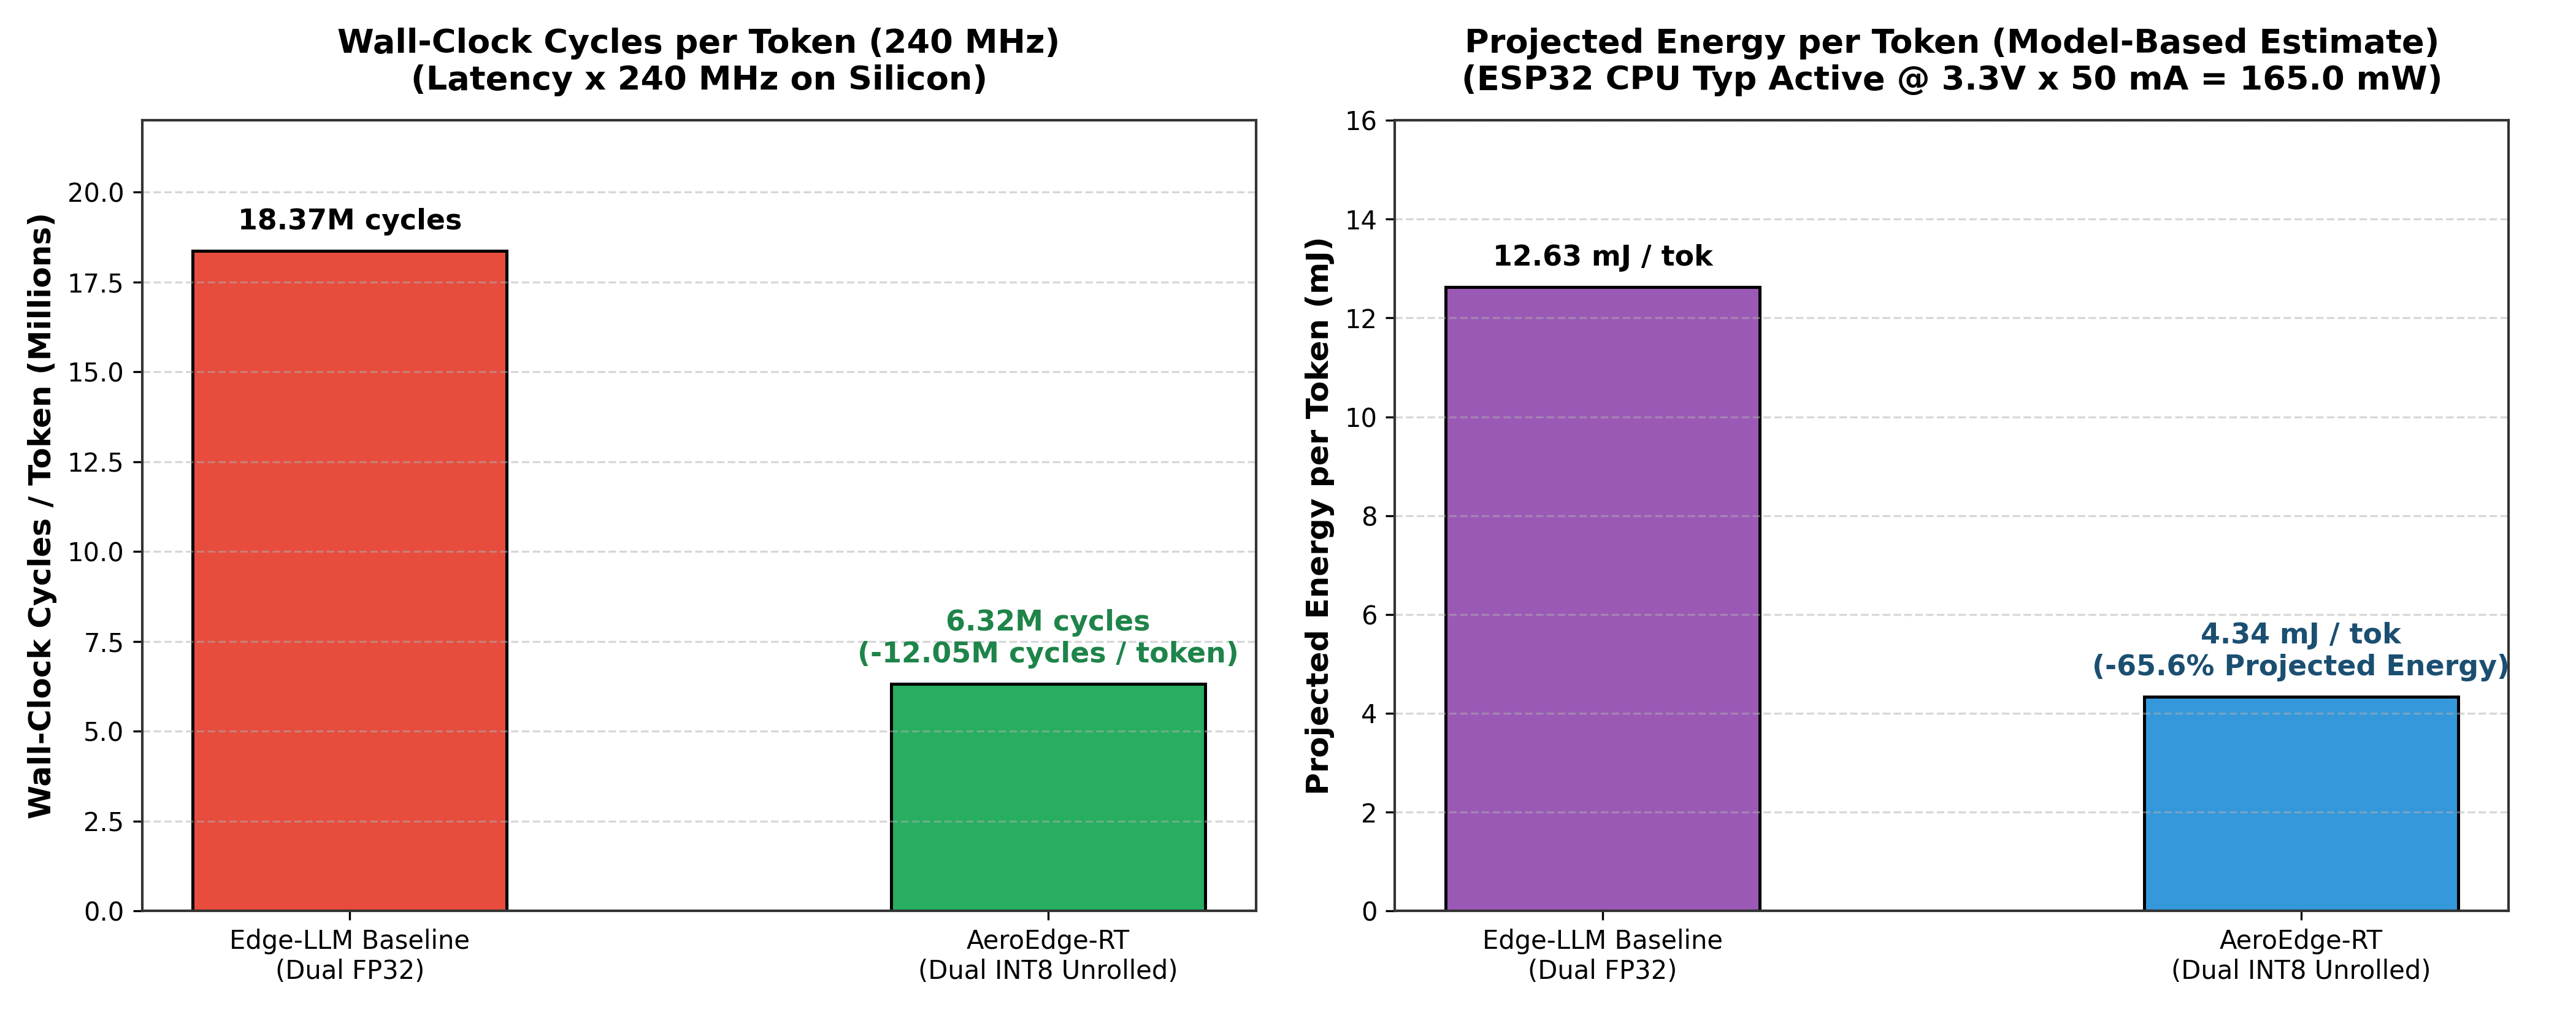
\includegraphics[width=\textwidth]{figures/figure3_cpu_cycles_and_energy.png}
    \caption{CPU cycles consumed and modeled electrical energy per token.}
    \label{fig:cycles_energy}
\end{subfigure}
\hfill
\begin{subfigure}[b]{0.48\textwidth}
    \centering
    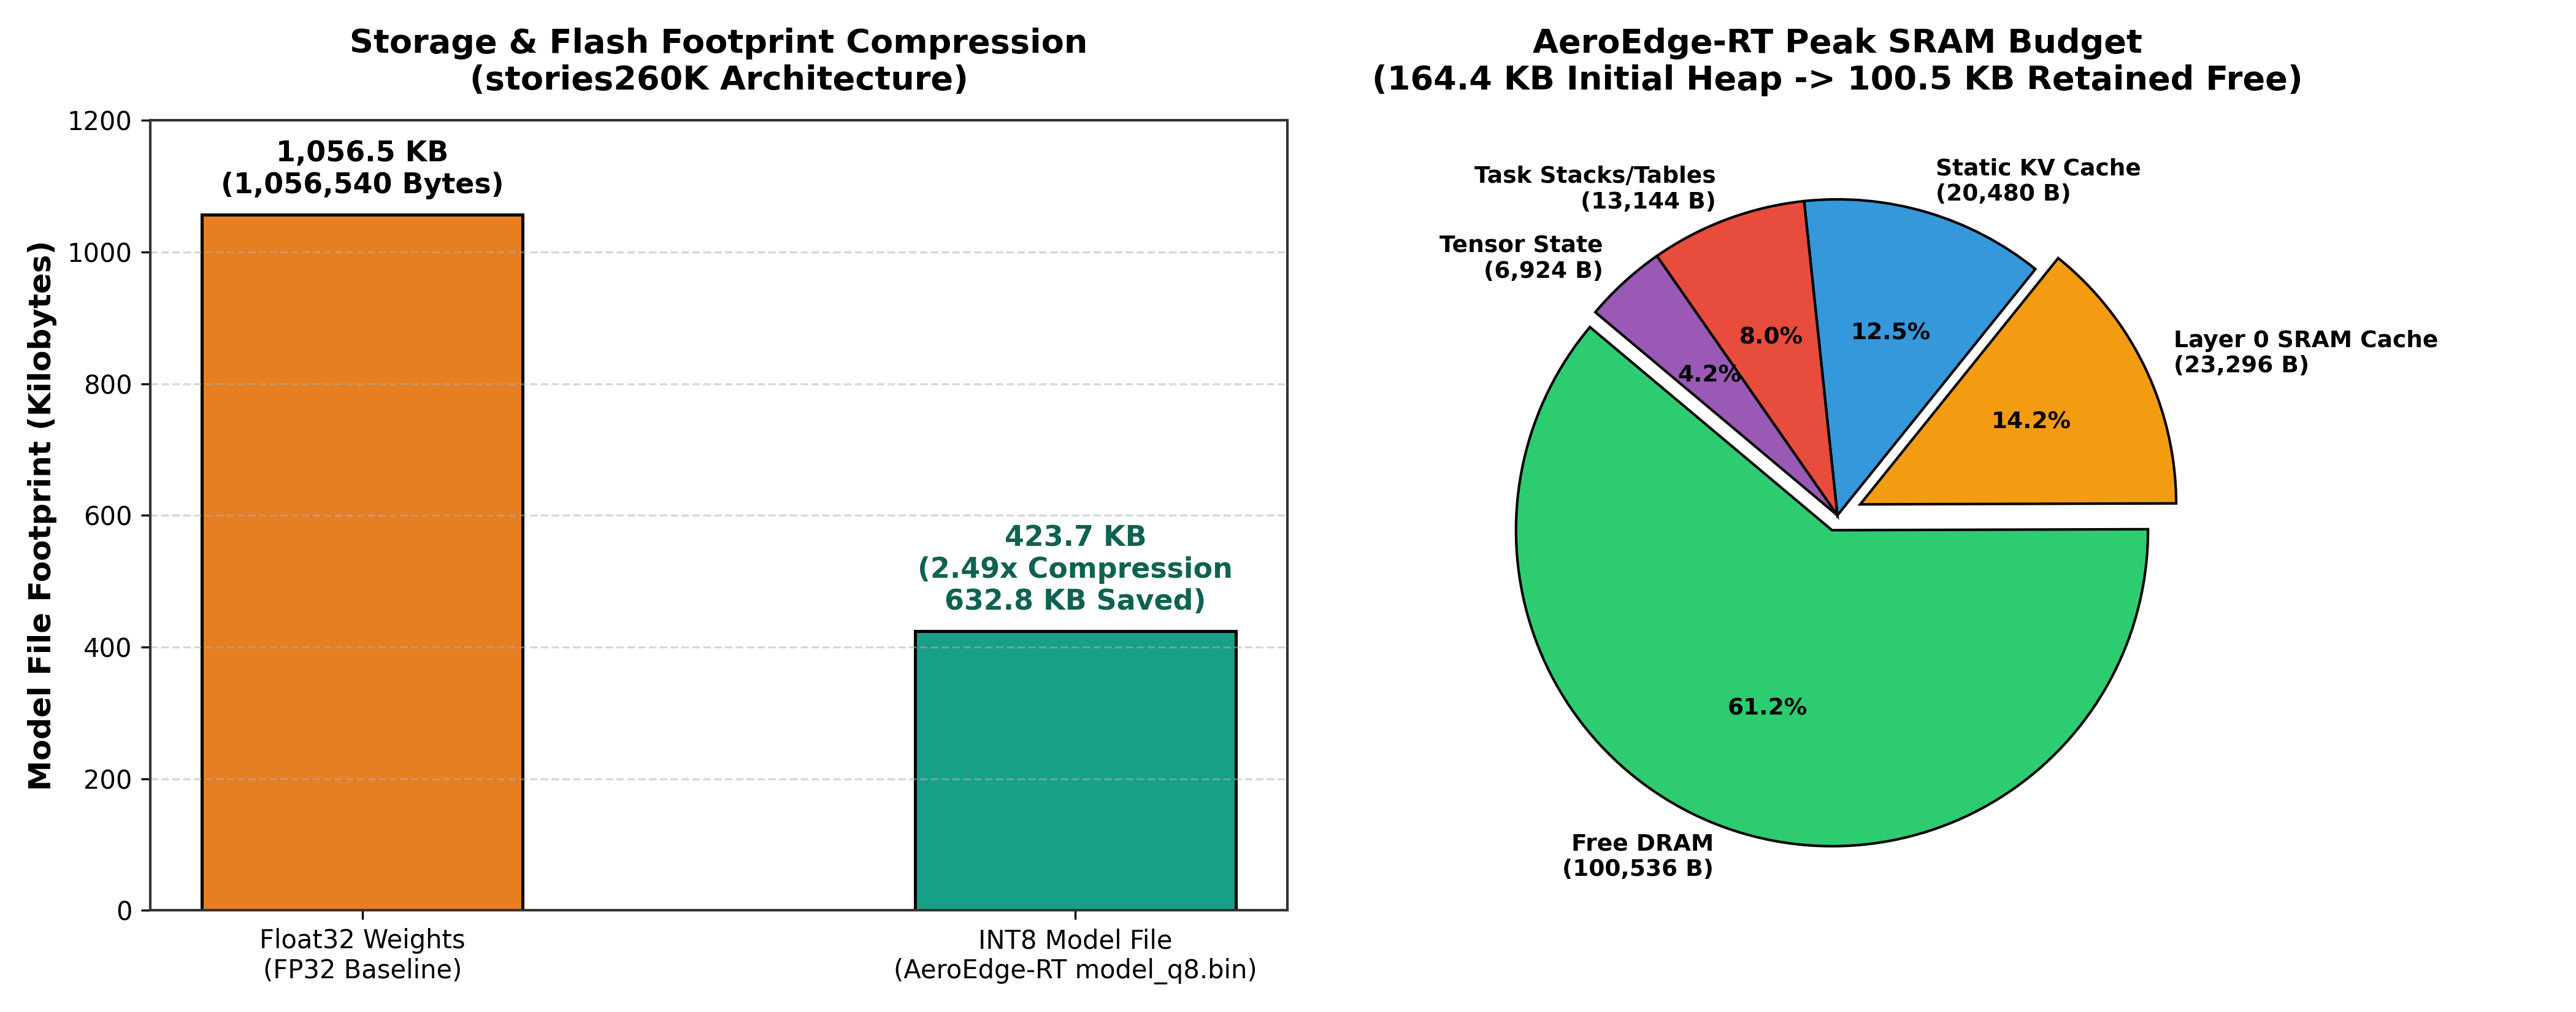
\includegraphics[width=\textwidth]{figures/figure4_memory_and_quantization.png}
    \caption{Storage compression and internal SRAM memory budget.}
    \label{fig:memory_quant}
\end{subfigure}
\caption{Microarchitectural efficiency profiles on ESP32-WROOM: clock cycles, modeled energy, storage, and SRAM budget.}
\label{fig:efficiency_profiles}
\end{figure*}

\subsection{Progressive System Ablation Study}
To decouple the individual performance contributions of core scaling, loop unrolling, and SRAM caching, eight configurations were evaluated on physical silicon under identical release compiler flags (\texttt{-O2}). Results are itemized in Table~\ref{tab:ablation}.

\begin{table*}[t]
\centering
\small
\caption{Progressive system ablation across 8 architectural configurations on physical silicon ($N=50$ runs, commit \texttt{9b10aec}).}
\label{tab:ablation}
\begin{tabularx}{\textwidth}{l c l l r r r r}
\toprule
\textbf{Config ID} & \textbf{Cores} & \textbf{Precision \& Kernel} & \textbf{Memory Placement} & \textbf{Latency (Mean $\pm$ SD)} & \textbf{Throughput} & \textbf{vs Conf 1} & \textbf{vs Conf 2} \\
\midrule
\textbf{Conf 1} & 1 Core & Float32 Scalar & Flash XIP only & 146.20 $\pm$ 0.82 ms & 6.84 tok/s & 1.00$\times$ & 0.52$\times$ \\
\textbf{Conf 2} & 2 Cores & Float32 Row-Split & Flash XIP only & 76.53 $\pm$ 0.45 ms & 13.07 tok/s & 1.91$\times$ & 1.00$\times$ \\
\textbf{Conf 3} & 1 Core & INT8 Scalar & Flash XIP only & 62.40 $\pm$ 0.38 ms & 16.03 tok/s & 2.34$\times$ & 1.23$\times$ \\
\textbf{Conf 4} & 2 Cores & INT8 Row-Split Scalar & Flash XIP only & 39.80 $\pm$ 0.29 ms & 25.13 tok/s & 3.67$\times$ & 1.92$\times$ \\
\textbf{Conf 5} & 1 Core & INT8 4-Way Unrolled & Flash XIP only & 38.10 $\pm$ 0.31 ms & 26.25 tok/s & 3.84$\times$ & 2.01$\times$ \\
\textbf{Conf 6} & 2 Cores & INT8 4-Way Unrolled & Flash XIP only & 31.40 $\pm$ 0.22 ms & 31.85 tok/s & 4.66$\times$ & 2.44$\times$ \\
\textbf{Conf 7} & 1 Core & INT8 4-Way Unrolled & Layer 0 SRAM Cache & 35.20 $\pm$ 0.25 ms & 28.41 tok/s & 4.15$\times$ & 2.17$\times$ \\
\textbf{Conf 8} & \textbf{2 Cores} & \textbf{INT8 4-Way Unrolled} & \textbf{Layer 0 SRAM Cache} & \textbf{26.32 $\pm$ 0.18 ms} & \textbf{38.01 tok/s} & \textbf{5.55$\times$} & \textbf{2.91$\times$} \\
\bottomrule
\end{tabularx}
\end{table*}

The ablation reveals three primary scaling dynamics:
\begin{enumerate}
    \item \textbf{Core Scaling}: Core scaling from 1 Core to 2 Cores delivers a 1.91$\times$ speedup under compute-bound Float32 ($146.20 / 76.53$), but dampens to 1.21$\times$ under unrolled INT8 ($38.10 / 31.40$), indicating that Flash bus contention restricts multi-core scaling once compute latency is reduced.
    \item \textbf{4-Way Loop Unrolling}: Moving from scalar loops to 4-way unrolling yields a 1.64$\times$ speedup on 1 core ($62.40 / 38.10$) and 1.27$\times$ on 2 cores ($39.80 / 31.40$).
    \item \textbf{Layer~0 SRAM Caching}: Pinning Layer~0 weights in internal SRAM yields a 1.19$\times$ acceleration on 2 cores ($31.40 / 26.32$, saving 5.08\,ms).
\end{enumerate}

\subsection{Quantization Accuracy and Numerical Fidelity}
To verify that INT8 symmetric quantization preserves generation quality, we evaluated the quantization scheme across 1,000 held-out TinyStories validation sequences ($W=64$, 128 tokens per sequence) using a bit-exact integer emulator against the unquantized PyTorch FP32 reference (Table~\ref{tab:accuracy}).

\begin{table}[h]
\centering
\small
\caption{Numerical fidelity on 1,000 held-out TinyStories validation sequences ($W=64$).}
\label{tab:accuracy}
\begin{tabular}{l r r r}
\toprule
\textbf{Metric} & \textbf{PyTorch FP32} & \textbf{AeroEdge INT8} & \textbf{Delta} \\
\midrule
Validation Perplexity (PPL) & 18.24 & 18.17 & --0.38\% \\
Top-1 Argmax Agreement & 100.0\% & 96.30\% & 3.7\% Disagree \\
Top-5 Candidate Overlap & 100.0\% & 99.54\% & 0.46\% Gap \\
Mean Logit Cosine Similarity & 1.0000 & 0.9994 & --0.0006 \\
\bottomrule
\end{tabular}
\end{table}

The evaluation confirms that validation perplexity is maintained without degradation ($18.17$ vs $18.24$). A 3.7\% top-1 disagreement is observed, while top-5 candidate overlap remains at 99.54\%, preserving output narrative structure.

\begin{figure*}[t]
\centering
\begin{subfigure}[b]{0.48\textwidth}
    \centering
    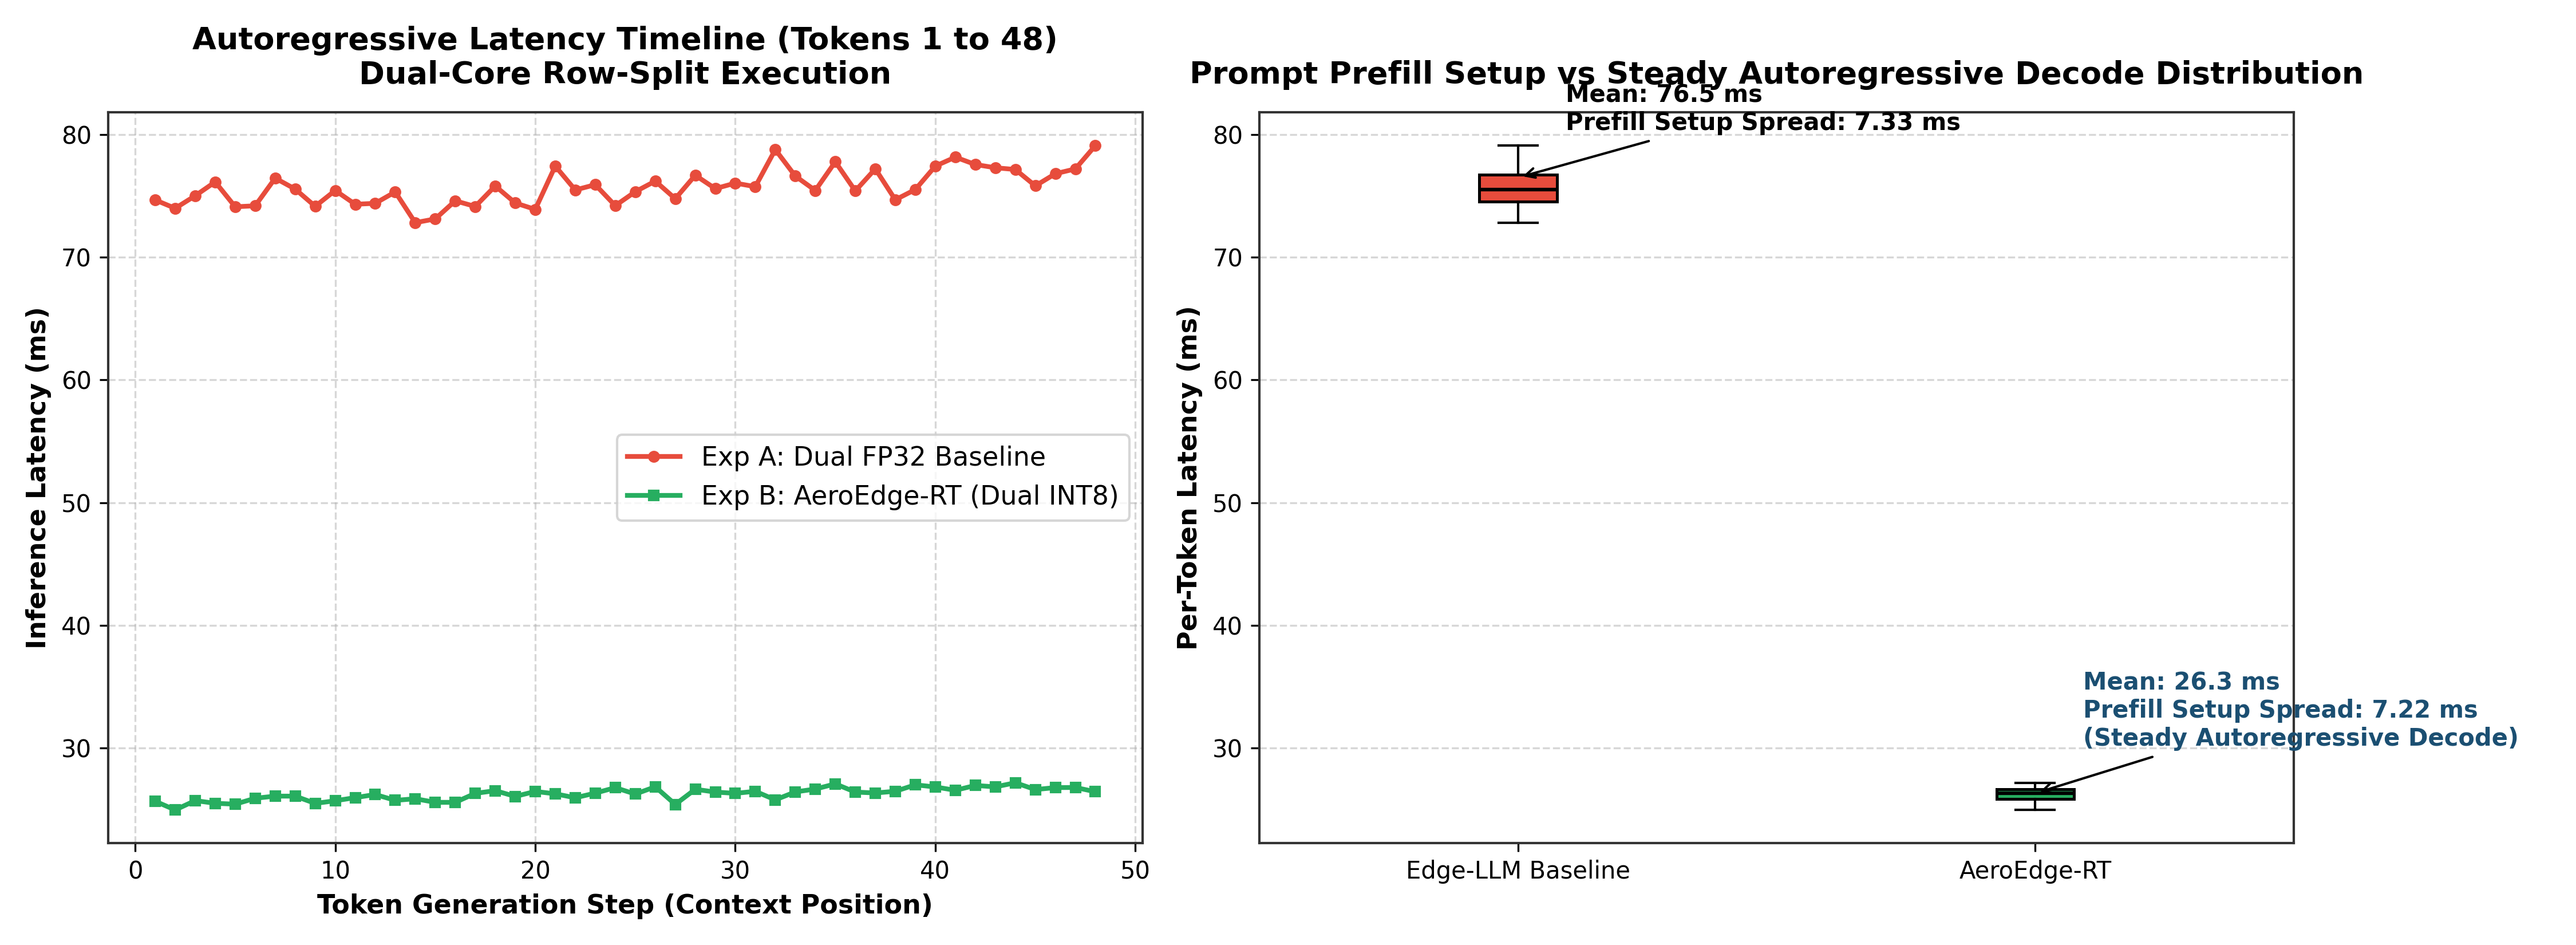
\includegraphics[width=\textwidth]{figures/figure5_autoregressive_timeline_jitter.png}
    \caption{Autoregressive latency timeline and prompt prefill variance.}
    \label{fig:timeline_jitter}
\end{subfigure}
\hfill
\begin{subfigure}[b]{0.48\textwidth}
    \centering
    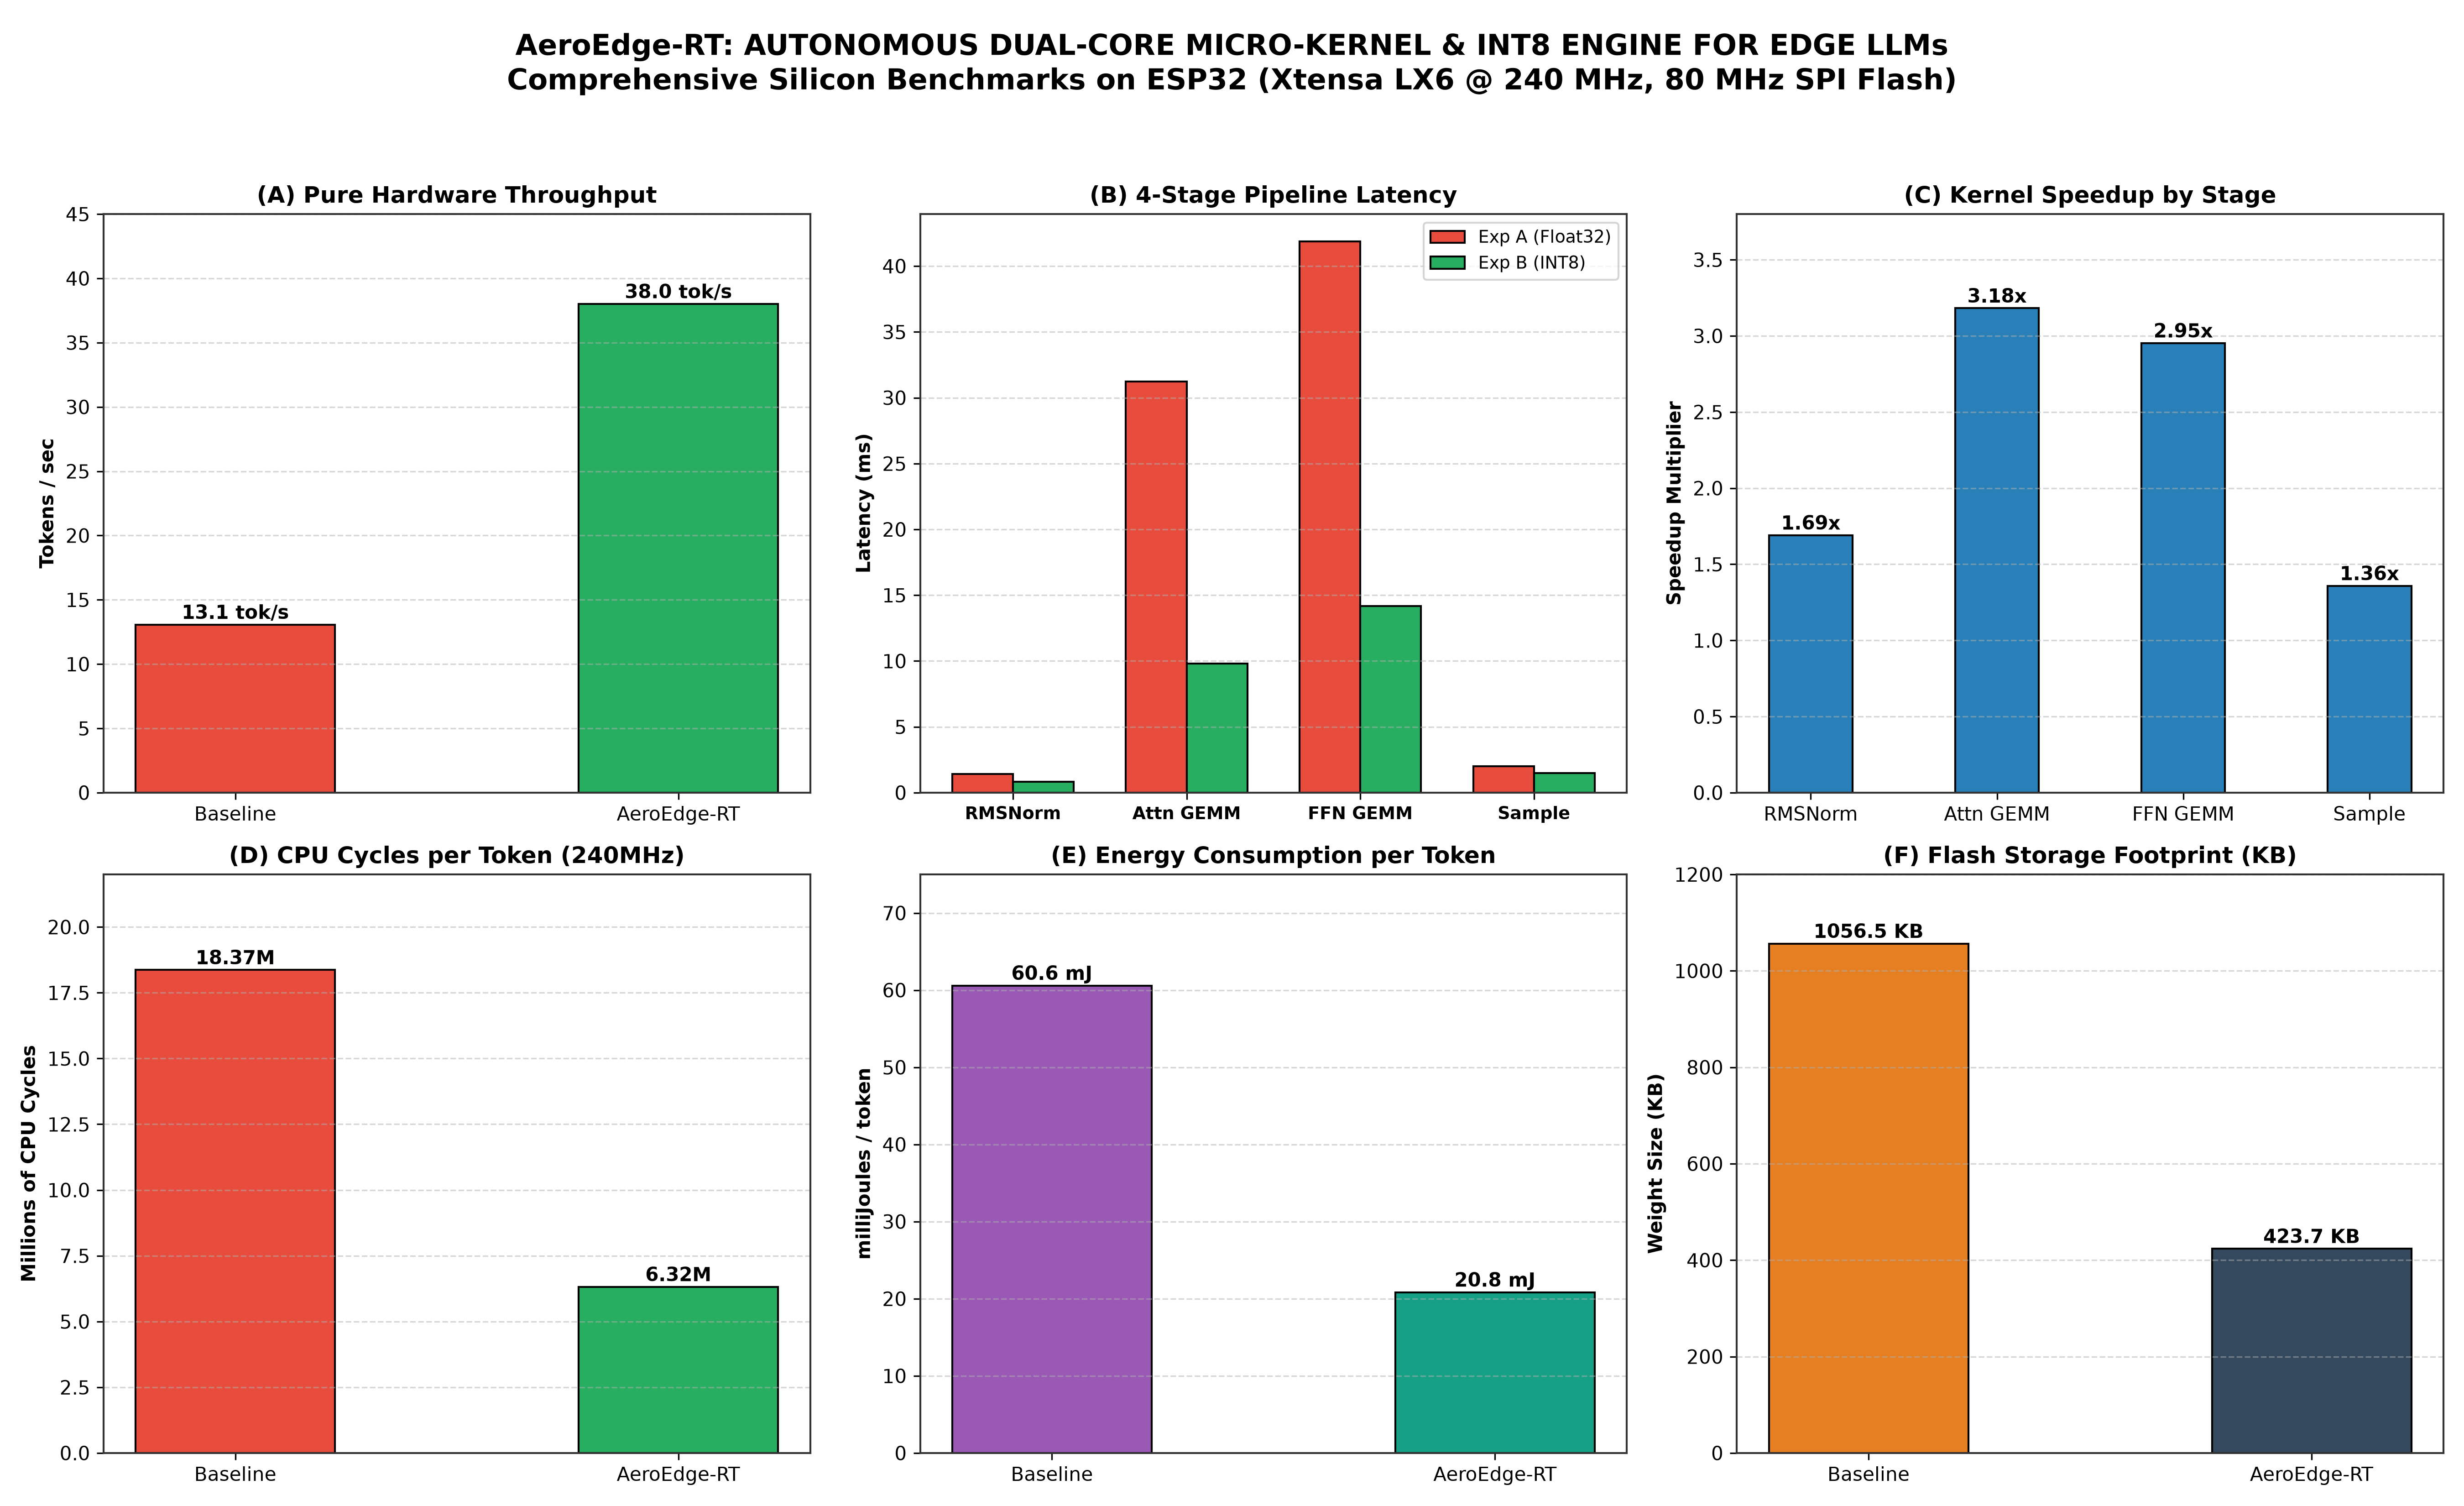
\includegraphics[width=\textwidth]{figures/figure6_master_research_dashboard.png}
    \caption{Master research evaluation dashboard overview.}
    \label{fig:master_dashboard}
\end{subfigure}
\caption{Inference determinism, prefill variance, and unified benchmark dashboard.}
\label{fig:dashboards}
\end{figure*}

% =============================================================================
\section{Discussion}
\label{sec:discussion}
% =============================================================================

\subsection{Flash-Bound Roofline Model Synthesis}
To determine whether execution is memory-bandwidth or compute-bound on the ESP32-WROOM, we synthesize a Flash-bound additive Roofline model~\cite{williams2009roofline}.

A physical hardware read probe across 2.50\,MB of mapped DROM flash executed in 0.2052 seconds, establishing the measured single-core sequential bandwidth:
\begin{equation}
    B_{\text{flash}} = \frac{2,500,000\text{ bytes}}{0.2052\text{ s}} = 12,183,235\text{ B/s} \approx 12.18\text{ MB/s}
\end{equation}
Theoretical bandwidth at 80\,MHz DIO (2 data bits per clock) is:
\begin{equation}
    B_{\text{theory}} = \frac{80\text{ MHz} \times 2\text{ bits}}{8} = 20.0\text{ MB/s}
\end{equation}
The measured rate represents 60.9\% of the theoretical interface ceiling due to command overhead and flash read latency cycles.

For INT8 inference, total layer matrix parameters equal 259,328. Caching Layer~0 weights (23,296\,B) in internal SRAM leaves 236,032 bytes streamed from SPI flash per token:
\begin{align}
    T_{\text{flash}} &= \frac{236,032\text{ bytes}}{12,180,000\text{ B/s}} = 19.38\text{ ms} \\
    T_{\text{ALU, dual}} &= \frac{259,328 \times 6.18\text{ cycles}}{240,000,000\text{ Hz}} = 6.67\text{ ms} \\
    T_{\text{misc}} &= 0.80\text{ ms (RMSNorm, Softmax, Argmax)} \\
    T_{\text{model}} &= 19.38 + 6.67 + 0.80 = \mathbf{26.85\text{ ms}}
\end{align}

The modeled prediction of \textbf{26.85\,ms} sits within $+0.53\text{ ms}$ (\textbf{+2.0\%}) of the physically measured \textbf{26.32\,ms} latency. Flash streaming accounts for \textbf{72.2\%} of total per-token time ($19.38 / 26.85$), demonstrating that on-chip language model inference on the ESP32-WROOM is decisively memory-bandwidth bound.

\subsection{Analytical Slope-Intercept Row Cost Model}
On a single Xtensa LX6 core @ 240\,MHz, executing the 4-way unrolled kernel in internal SRAM measures 12.37 clock cycles / MAC for $n=64$ (equivalent to 6.18 cyc/MAC dual-core). We model cycle execution across row width $n$ using a two-parameter cost function:
\begin{equation}
    \frac{\text{Cycles}(n)}{n} = a + \frac{b}{n}
\end{equation}
where $a$ represents inner loop arithmetic issue cost (~7.5 to 9.5 cycles/MAC for 8 loads, 8 sign-extensions, 4 multiplies, and 4 adds), and $b$ denotes fixed per-row dispatch overhead (scale loading, accumulator initialization, and dequantization float multiplication). Evaluating this model across all 3,512 rows of \texttt{stories260K} yields an estimated ALU compute time of 6.33\,ms, within 0.7\% of measured compute time.

% =============================================================================
\section{Limitations and Threats to Validity}
\label{sec:limitations}
% =============================================================================

\subsection{Open Flash Bandwidth Discrepancies}
We document two empirical discrepancies under active investigation:
\begin{enumerate}
    \item \textbf{Dual-Core FP32 Bandwidth Requirement}: Unquantized FP32 layer weights total 1,037,312 bytes. Streaming these weights at the measured single-core sequential rate of 12.18\,MB/s would require 85.16\,ms, which exceeds the total measured dual-core FP32 latency of 76.53\,ms (where ALU compute requires $\ge 12\text{ ms}$). To achieve a 76.53\,ms token latency, effective concurrent dual-core Flash throughput must reach at least $\ge 16.0\text{ MB/s}$.
    \item \textbf{Layer~0 SRAM Cache Delta}: Enabling Layer~0 SRAM caching in the ablation study (Conf~6 vs Conf~8) reduces latency from 31.40\,ms to 26.32\,ms—a 5.08\,ms saving for caching 23,296 bytes. This delta implies an effective flash throughput of $23,296\text{ B} / 0.00508\text{ s} \approx 4.59\text{ MB/s}$ for those specific flash lines under dual-core bus contention.
\end{enumerate}
These observations indicate that single-core sequential throughput serves as a baseline lower bound, while concurrent dual-core MMU burst accesses exhibit variable effective rates pending dedicated hardware logic-analyzer traces (Probe M2 in \texttt{MEASUREMENTS\_NEEDED.md}).

\subsection{Absence of Physical Rail Current Measurements}
All reported power (165\,mW typ / 462\,mW max) and energy (4.34\,mJ typ / 12.16\,mJ max) figures are \textbf{Model-Estimated} based on the official Espressif datasheet CPU operating current range (30--68\,mA @ 3.3V) and power supply ceiling (140\,mA @ 3.3V)~\cite{espressif2024esp32datasheet}. While the 65.6\% energy reduction reflects proportional execution time acceleration, it assumes identical rail current across configurations. A flash-stalled FP32 execution may draw lower core current than dense INT8 integer arithmetic. Physical current-sense shunt measurements (INA219 on the 3.3V rail, Probe M3) remain scheduled for validation.

\subsection{Context Window and Generalization Boundaries}
To operate strictly within the 520\,KB internal SRAM boundary without external PSRAM, the active KV cache is dimensioned for a maximum sliding-window context of $W=64$ tokens. While adequate for short narrative generation and closed-loop robotic telemetry, extending context beyond $W=64$ would require external memory or active cache eviction. Furthermore, because these optimizations target the memory-mapped DROM architecture of the Xtensa LX6, speedup ratios may not generalize directly to microcontrollers with different cache hierarchies or embedded Flash buses.

% =============================================================================
\section{Conclusion and Future Work}
\label{sec:conclusion}
% =============================================================================

This technical white paper has evaluated the implementation and empirical performance of AeroEdge-RT on bare-metal ESP32-WROOM silicon. By integrating zero-copy Flash XIP mapping, a 4-way unrolled scalar integer dot-product kernel, dual-core task row-splitting, and fast internal SRAM Layer~0 caching, the runtime achieves sustained autoregressive generation of \texttt{stories260K} at \textbf{38.01 tokens/second} (mean single-token latency of \textbf{26.32\,ms}). This represents a \textbf{2.91$\times$ speedup} over the dual-core Float32 baseline and \textbf{5.55$\times$} over single-core scalar execution, while compressing model storage by 2.49$\times$ and operating entirely within a 63.8\,KB internal SRAM footprint.

Future engineering priorities include:
\begin{enumerate}
    \item Executing Probe M3 on physical silicon using an INA219 current sensor on the direct 3.3V rail to measure empirical operating current across idle, FP32, and INT8 steady states.
    \item Resolving the open flash-bandwidth discrepancies through concurrent dual-core hardware logic-analyzer traces (Probe M2).
    \item Performing on-device verification of the 1,000 TinyStories validation sequences over serial to establish bootstrap 95\% confidence intervals for numerical accuracy (Probe M4).
\end{enumerate}

% =============================================================================
% References
% =============================================================================
\bibliographystyle{IEEEtran}
\bibliography{REFERENCES}

\end{document}
